\documentclass[a4paper]{article}
\usepackage[]{graphicx}\usepackage[]{xcolor}
% maxwidth is the original width if it is less than linewidth
% otherwise use linewidth (to make sure the graphics do not exceed the margin)
\makeatletter
\def\maxwidth{ %
  \ifdim\Gin@nat@width>\linewidth
    \linewidth
  \else
    \Gin@nat@width
  \fi
}
\makeatother

\definecolor{fgcolor}{rgb}{0.345, 0.345, 0.345}
\newcommand{\hlnum}[1]{\textcolor[rgb]{0.686,0.059,0.569}{#1}}%
\newcommand{\hlstr}[1]{\textcolor[rgb]{0.192,0.494,0.8}{#1}}%
\newcommand{\hlcom}[1]{\textcolor[rgb]{0.678,0.584,0.686}{\textit{#1}}}%
\newcommand{\hlopt}[1]{\textcolor[rgb]{0,0,0}{#1}}%
\newcommand{\hlstd}[1]{\textcolor[rgb]{0.345,0.345,0.345}{#1}}%
\newcommand{\hlkwa}[1]{\textcolor[rgb]{0.161,0.373,0.58}{\textbf{#1}}}%
\newcommand{\hlkwb}[1]{\textcolor[rgb]{0.69,0.353,0.396}{#1}}%
\newcommand{\hlkwc}[1]{\textcolor[rgb]{0.333,0.667,0.333}{#1}}%
\newcommand{\hlkwd}[1]{\textcolor[rgb]{0.737,0.353,0.396}{\textbf{#1}}}%
\let\hlipl\hlkwb

\usepackage{framed}
\makeatletter
\newenvironment{kframe}{%
 \def\at@end@of@kframe{}%
 \ifinner\ifhmode%
  \def\at@end@of@kframe{\end{minipage}}%
  \begin{minipage}{\columnwidth}%
 \fi\fi%
 \def\FrameCommand##1{\hskip\@totalleftmargin \hskip-\fboxsep
 \colorbox{shadecolor}{##1}\hskip-\fboxsep
     % There is no \\@totalrightmargin, so:
     \hskip-\linewidth \hskip-\@totalleftmargin \hskip\columnwidth}%
 \MakeFramed {\advance\hsize-\width
   \@totalleftmargin\z@ \linewidth\hsize
   \@setminipage}}%
 {\par\unskip\endMakeFramed%
 \at@end@of@kframe}
\makeatother

\definecolor{shadecolor}{rgb}{.97, .97, .97}
\definecolor{messagecolor}{rgb}{0, 0, 0}
\definecolor{warningcolor}{rgb}{1, 0, 1}
\definecolor{errorcolor}{rgb}{1, 0, 0}
\newenvironment{knitrout}{}{} % an empty environment to be redefined in TeX

\usepackage{alltt}
\newcommand{\SweaveOpts}[1]{}  % do not interfere with LaTeX
\newcommand{\SweaveInput}[1]{} % because they are not real TeX commands
\newcommand{\Sexpr}[1]{}       % will only be parsed by R




\usepackage[utf8]{inputenc}
%\usepackage[ngerman]{babel}
\usepackage{a4wide,paralist}
\usepackage{amsmath, amssymb, xfrac, amsthm}
\usepackage{dsfont}
%\usepackage[usenames,dvipsnames]{xcolor}
\usepackage{amsfonts}
\usepackage{graphicx}
\usepackage{caption}
\usepackage{subcaption}
\usepackage{framed}
\usepackage{multirow}
\usepackage{bytefield}
\usepackage{csquotes}
\usepackage[breakable, theorems, skins]{tcolorbox}
\usepackage{hyperref}
\usepackage{cancel}
\usepackage{bm}


% This file is included in slides and exercises

% Rarely used fontstyle for R packages, used only in 
% - forests/slides-forests-benchmark.tex
% - exercises/single-exercises/methods_l_1.Rnw
% - slides/cart/attic/slides_extra_trees.Rnw
\newcommand{\pkg}[1]{{\fontseries{b}\selectfont #1}}

% Spacing helpers, used often (mostly in exercises for \dlz)
\newcommand{\lz}{\vspace{0.5cm}} % vertical space (used often in slides)
\newcommand{\dlz}{\vspace{1cm}}  % double vertical space (used often in exercises, never in slides)

% Don't know if this is used or needed, remove?
% textcolor that works in mathmode
% https://tex.stackexchange.com/a/261480
% Used e.g. in forests/slides-forests-bagging.tex
% [...] \textcolor{blue}{\tfrac{1}{M}\sum^M_{m} [...]
% \makeatletter
% \renewcommand*{\@textcolor}[3]{%
%   \protect\leavevmode
%   \begingroup
%     \color#1{#2}#3%
%   \endgroup
% }
% \makeatother


\tcbset{enhanced}

\DeclareRobustCommand{\mybox}[2][gray!20]{%
	\iffalse
	\begin{tcolorbox}[   %% Adjust the following parameters at will.
		breakable,
		left=0pt,
		right=0pt,
		top=0pt,
		bottom=0pt,
		colback=#1,
		colframe=#1,
		width=\dimexpr\linewidth\relax,
		enlarge left by=0mm,
		boxsep=5pt,
		arc=0pt,outer arc=0pt,
		]
		#2
	\end{tcolorbox}
	\fi
}

\DeclareRobustCommand{\myboxshow}[2][gray!20]{%
%	\iffalse
	\begin{tcolorbox}[   %% Adjust the following parameters at will.
		breakable,
		left=0pt,
		right=0pt,
		top=0pt,
		bottom=0pt,
		colback=#1,
		colframe=#1,
		width=\dimexpr\linewidth\relax,
		enlarge left by=0mm,
		boxsep=5pt,
		arc=0pt,outer arc=0pt,
		]
		#2
	\end{tcolorbox}
%	\fi
}


%exercise numbering
\renewcommand{\theenumi}{(\alph{enumi})}
\renewcommand{\theenumii}{\roman{enumii}}
\renewcommand\labelenumi{\theenumi}


\font \sfbold=cmssbx10

\setlength{\oddsidemargin}{0cm} \setlength{\textwidth}{16cm}


\sloppy
\parindent0em
\parskip0.5em
\topmargin-2.3 cm
\textheight25cm
\textwidth17.5cm
\oddsidemargin-0.8cm
\pagestyle{empty}

\newcommand{\kopf}[1]{
\hrule
\vspace{.15cm}
\begin{minipage}{\textwidth}
%akwardly i had to put \" here to make it compile correctly
	{\sf\bf Optimization in Machine Learning \hfill Exercise sheet #1\\
	 \url{https://slds-lmu.github.io/website_optimization/} \hfill WS 2024/2025}
\end{minipage}
\vspace{.05cm}
\hrule
\vspace{1cm}}

\newcommand{\kopfic}[1]{
\hrule
\vspace{.15cm}
\begin{minipage}{\textwidth}
%akwardly i had to put \" here to make it compile correctly
	{\sf\bf Optimization in Machine Learning \hfill Live Session #1\\
	 \url{https://slds-lmu.github.io/website_optimization/} \hfill WS 2024/2025}
\end{minipage}
\vspace{.05cm}
\hrule
\vspace{1cm}}

\newcommand{\kopfsl}[1]{
\hrule
\vspace{.15cm}
\begin{minipage}{\textwidth}
%akwardly i had to put \" here to make it compile correctly
	{\sf\bf Optimization in Machine Learning \hfill Exercise sheet #1\\
	 \url{https://slds-lmu.github.io/website_optimization/} \hfill WS 2024/2025}
\end{minipage}
\vspace{.05cm}
\hrule
\vspace{1cm}}

\newenvironment{allgemein}
	{\noindent}{\vspace{1cm}}

\newcounter{aufg}
\newenvironment{aufgabe}[1]
	{\refstepcounter{aufg}\textbf{Exercise \arabic{aufg}: #1}\\ \noindent}
	{\vspace{0.5cm}}

\newcounter{loes}
\newenvironment{loesung}[1]
	{\refstepcounter{loes}\textbf{Solution \arabic{loes}: #1}\\ \noindent}
	{\bigskip}
	
\newenvironment{bonusaufgabe}
	{\refstepcounter{aufg}\textbf{Exercise \arabic{aufg}*\footnote{This
	is a bonus exercise.}:}\\ \noindent}
	{\vspace{0.5cm}}

\newenvironment{bonusloesung}
	{\refstepcounter{loes}\textbf{Solution \arabic{loes}*:}\\\noindent}
	{\bigskip}

% dependencies: amsmath, amssymb, dsfont
% math spaces
\ifdefined\N
\renewcommand{\N}{\mathds{N}} % N, naturals
\else \newcommand{\N}{\mathds{N}} \fi
\newcommand{\Z}{\mathds{Z}} % Z, integers
\newcommand{\Q}{\mathds{Q}} % Q, rationals
\newcommand{\R}{\mathds{R}} % R, reals
\ifdefined\C
\renewcommand{\C}{\mathds{C}} % C, complex
\else \newcommand{\C}{\mathds{C}} \fi
\newcommand{\continuous}{\mathcal{C}} % C, space of continuous functions
\newcommand{\M}{\mathcal{M}} % machine numbers
\newcommand{\epsm}{\epsilon_m} % maximum error

% counting / finite sets
\newcommand{\setzo}{\{0, 1\}} % set 0, 1
\newcommand{\setmp}{\{-1, +1\}} % set -1, 1
\newcommand{\unitint}{[0, 1]} % unit interval

% basic math stuff
\newcommand{\xt}{\tilde x} % x tilde
\DeclareMathOperator*{\argmax}{arg\,max} % argmax
\DeclareMathOperator*{\argmin}{arg\,min} % argmin
\newcommand{\argminlim}{\mathop{\mathrm{arg\,min}}\limits} % argmax with limits
\newcommand{\argmaxlim}{\mathop{\mathrm{arg\,max}}\limits} % argmin with limits
\newcommand{\sign}{\operatorname{sign}} % sign, signum
\newcommand{\I}{\mathbb{I}} % I, indicator
\newcommand{\order}{\mathcal{O}} % O, order
\newcommand{\bigO}{\mathcal{O}} % Big-O Landau
\newcommand{\littleo}{{o}} % Little-o Landau
\newcommand{\pd}[2]{\frac{\partial{#1}}{\partial #2}} % partial derivative
\newcommand{\floorlr}[1]{\left\lfloor #1 \right\rfloor} % floor
\newcommand{\ceillr}[1]{\left\lceil #1 \right\rceil} % ceiling
\newcommand{\indep}{\perp \!\!\! \perp} % independence symbol

% sums and products
\newcommand{\sumin}{\sum\limits_{i=1}^n} % summation from i=1 to n
\newcommand{\sumim}{\sum\limits_{i=1}^m} % summation from i=1 to m
\newcommand{\sumjn}{\sum\limits_{j=1}^n} % summation from j=1 to p
\newcommand{\sumjp}{\sum\limits_{j=1}^p} % summation from j=1 to p
\newcommand{\sumik}{\sum\limits_{i=1}^k} % summation from i=1 to k
\newcommand{\sumkg}{\sum\limits_{k=1}^g} % summation from k=1 to g
\newcommand{\sumjg}{\sum\limits_{j=1}^g} % summation from j=1 to g
\newcommand{\summM}{\sum\limits_{m=1}^M} % summation from m=1 to M
\newcommand{\meanin}{\frac{1}{n} \sum\limits_{i=1}^n} % mean from i=1 to n
\newcommand{\meanim}{\frac{1}{m} \sum\limits_{i=1}^m} % mean from i=1 to n
\newcommand{\meankg}{\frac{1}{g} \sum\limits_{k=1}^g} % mean from k=1 to g
\newcommand{\meanmM}{\frac{1}{M} \sum\limits_{m=1}^M} % mean from m=1 to M
\newcommand{\prodin}{\prod\limits_{i=1}^n} % product from i=1 to n
\newcommand{\prodkg}{\prod\limits_{k=1}^g} % product from k=1 to g
\newcommand{\prodjp}{\prod\limits_{j=1}^p} % product from j=1 to p

% linear algebra
\newcommand{\one}{\bm{1}} % 1, unitvector
\newcommand{\zero}{\mathbf{0}} % 0-vector
\newcommand{\id}{\bm{I}} % I, identity
\newcommand{\diag}{\operatorname{diag}} % diag, diagonal
\newcommand{\trace}{\operatorname{tr}} % tr, trace
\newcommand{\spn}{\operatorname{span}} % span
\newcommand{\scp}[2]{\left\langle #1, #2 \right\rangle} % <.,.>, scalarproduct
\newcommand{\mat}[1]{\begin{pmatrix} #1 \end{pmatrix}} % short pmatrix command
\newcommand{\Amat}{\mathbf{A}} % matrix A
\newcommand{\Deltab}{\mathbf{\Delta}} % error term for vectors

% basic probability + stats
\renewcommand{\P}{\mathds{P}} % P, probability
\newcommand{\E}{\mathds{E}} % E, expectation
\newcommand{\var}{\mathsf{Var}} % Var, variance
\newcommand{\cov}{\mathsf{Cov}} % Cov, covariance
\newcommand{\corr}{\mathsf{Corr}} % Corr, correlation
\newcommand{\normal}{\mathcal{N}} % N of the normal distribution
\newcommand{\iid}{\overset{i.i.d}{\sim}} % dist with i.i.d superscript
\newcommand{\distas}[1]{\overset{#1}{\sim}} % ... is distributed as ...

% machine learning
\newcommand{\Xspace}{\mathcal{X}} % X, input space
\newcommand{\Yspace}{\mathcal{Y}} % Y, output space
\newcommand{\Zspace}{\mathcal{Z}} % Z, space of sampled datapoints
\newcommand{\nset}{\{1, \ldots, n\}} % set from 1 to n
\newcommand{\pset}{\{1, \ldots, p\}} % set from 1 to p
\newcommand{\gset}{\{1, \ldots, g\}} % set from 1 to g
\newcommand{\Pxy}{\mathbb{P}_{xy}} % P_xy
\newcommand{\Exy}{\mathbb{E}_{xy}} % E_xy: Expectation over random variables xy
\newcommand{\xv}{\mathbf{x}} % vector x (bold)
\newcommand{\xtil}{\tilde{\mathbf{x}}} % vector x-tilde (bold)
\newcommand{\yv}{\mathbf{y}} % vector y (bold)
\newcommand{\xy}{(\xv, y)} % observation (x, y)
\newcommand{\xvec}{\left(x_1, \ldots, x_p\right)^\top} % (x1, ..., xp)
\newcommand{\Xmat}{\mathbf{X}} % Design matrix
\newcommand{\allDatasets}{\mathds{D}} % The set of all datasets
\newcommand{\allDatasetsn}{\mathds{D}_n}  % The set of all datasets of size n
\newcommand{\D}{\mathcal{D}} % D, data
\newcommand{\Dn}{\D_n} % D_n, data of size n
\newcommand{\Dtrain}{\mathcal{D}_{\text{train}}} % D_train, training set
\newcommand{\Dtest}{\mathcal{D}_{\text{test}}} % D_test, test set
\newcommand{\xyi}[1][i]{\left(\xv^{(#1)}, y^{(#1)}\right)} % (x^i, y^i), i-th observation
\newcommand{\Dset}{\left( \xyi[1], \ldots, \xyi[n]\right)} % {(x1,y1)), ..., (xn,yn)}, data
\newcommand{\defAllDatasetsn}{(\Xspace \times \Yspace)^n} % Def. of the set of all datasets of size n
\newcommand{\defAllDatasets}{\bigcup_{n \in \N}(\Xspace \times \Yspace)^n} % Def. of the set of all datasets
\newcommand{\xdat}{\left\{ \xv^{(1)}, \ldots, \xv^{(n)}\right\}} % {x1, ..., xn}, input data
\newcommand{\ydat}{\left\{ \yv^{(1)}, \ldots, \yv^{(n)}\right\}} % {y1, ..., yn}, input data
\newcommand{\yvec}{\left(y^{(1)}, \hdots, y^{(n)}\right)^\top} % (y1, ..., yn), vector of outcomes
\newcommand{\greekxi}{\xi} % Greek letter xi
\renewcommand{\xi}[1][i]{\xv^{(#1)}} % x^i, i-th observed value of x
\newcommand{\yi}[1][i]{y^{(#1)}} % y^i, i-th observed value of y
\newcommand{\xivec}{\left(x^{(i)}_1, \ldots, x^{(i)}_p\right)^\top} % (x1^i, ..., xp^i), i-th observation vector
\newcommand{\xj}{\xv_j} % x_j, j-th feature
\newcommand{\xjvec}{\left(x^{(1)}_j, \ldots, x^{(n)}_j\right)^\top} % (x^1_j, ..., x^n_j), j-th feature vector
\newcommand{\phiv}{\mathbf{\phi}} % Basis transformation function phi
\newcommand{\phixi}{\mathbf{\phi}^{(i)}} % Basis transformation of xi: phi^i := phi(xi)

%%%%%% ml - models general
\newcommand{\lamv}{\bm{\lambda}} % lambda vector, hyperconfiguration vector
\newcommand{\Lam}{\bm{\Lambda}}	 % Lambda, space of all hpos
% Inducer / Inducing algorithm
\newcommand{\preimageInducer}{\left(\defAllDatasets\right)\times\Lam} % Set of all datasets times the hyperparameter space
\newcommand{\preimageInducerShort}{\allDatasets\times\Lam} % Set of all datasets times the hyperparameter space
% Inducer / Inducing algorithm
\newcommand{\ind}{\mathcal{I}} % Inducer, inducing algorithm, learning algorithm

% continuous prediction function f
\newcommand{\ftrue}{f_{\text{true}}}  % True underlying function (if a statistical model is assumed)
\newcommand{\ftruex}{\ftrue(\xv)} % True underlying function (if a statistical model is assumed)
\newcommand{\fx}{f(\xv)} % f(x), continuous prediction function
\newcommand{\fdomains}{f: \Xspace \rightarrow \R^g} % f with domain and co-domain
\newcommand{\Hspace}{\mathcal{H}} % hypothesis space where f is from
\newcommand{\fbayes}{f^{\ast}} % Bayes-optimal model
\newcommand{\fxbayes}{f^{\ast}(\xv)} % Bayes-optimal model
\newcommand{\fkx}[1][k]{f_{#1}(\xv)} % f_j(x), discriminant component function
\newcommand{\fh}{\hat{f}} % f hat, estimated prediction function
\newcommand{\fxh}{\fh(\xv)} % fhat(x)
\newcommand{\fxt}{f(\xv ~|~ \thetav)} % f(x | theta)
\newcommand{\fxi}{f\left(\xv^{(i)}\right)} % f(x^(i))
\newcommand{\fxih}{\hat{f}\left(\xv^{(i)}\right)} % f(x^(i))
\newcommand{\fxit}{f\left(\xv^{(i)} ~|~ \thetav\right)} % f(x^(i) | theta)
\newcommand{\fhD}{\fh_{\D}} % fhat_D, estimate of f based on D
\newcommand{\fhDtrain}{\fh_{\Dtrain}} % fhat_Dtrain, estimate of f based on D
\newcommand{\fhDnlam}{\fh_{\Dn, \lamv}} %model learned on Dn with hp lambda
\newcommand{\fhDlam}{\fh_{\D, \lamv}} %model learned on D with hp lambda
\newcommand{\fhDnlams}{\fh_{\Dn, \lamv^\ast}} %model learned on Dn with optimal hp lambda
\newcommand{\fhDlams}{\fh_{\D, \lamv^\ast}} %model learned on D with optimal hp lambda

% discrete prediction function h
\newcommand{\hx}{h(\xv)} % h(x), discrete prediction function
\newcommand{\hh}{\hat{h}} % h hat
\newcommand{\hxh}{\hat{h}(\xv)} % hhat(x)
\newcommand{\hxt}{h(\xv | \thetav)} % h(x | theta)
\newcommand{\hxi}{h\left(\xi\right)} % h(x^(i))
\newcommand{\hxit}{h\left(\xi ~|~ \thetav\right)} % h(x^(i) | theta)
\newcommand{\hbayes}{h^{\ast}} % Bayes-optimal classification model
\newcommand{\hxbayes}{h^{\ast}(\xv)} % Bayes-optimal classification model

% yhat
\newcommand{\yh}{\hat{y}} % yhat for prediction of target
\newcommand{\yih}{\hat{y}^{(i)}} % yhat^(i) for prediction of ith targiet
\newcommand{\resi}{\yi- \yih}

% theta
\newcommand{\thetah}{\hat{\theta}} % theta hat
\newcommand{\thetav}{\bm{\theta}} % theta vector
\newcommand{\thetavh}{\bm{\hat\theta}} % theta vector hat
\newcommand{\thetat}[1][t]{\thetav^{[#1]}} % theta^[t] in optimization
\newcommand{\thetatn}[1][t]{\thetav^{[#1 +1]}} % theta^[t+1] in optimization
\newcommand{\thetahDnlam}{\thetavh_{\Dn, \lamv}} %theta learned on Dn with hp lambda
\newcommand{\thetahDlam}{\thetavh_{\D, \lamv}} %theta learned on D with hp lambda
\newcommand{\mint}{\min_{\thetav \in \Theta}} % min problem theta
\newcommand{\argmint}{\argmin_{\thetav \in \Theta}} % argmin theta
% LS 29.10.2024 addin thetab back for now because apparently this broke and nobody updated slides to reflect thetab -> thetav changes?
\newcommand{\thetab}{\bm{\theta}} % theta vector


% densities + probabilities
% pdf of x
\newcommand{\pdf}{p} % p
\newcommand{\pdfx}{p(\xv)} % p(x)
\newcommand{\pixt}{\pi(\xv~|~ \thetav)} % pi(x|theta), pdf of x given theta
\newcommand{\pixit}[1][i]{\pi\left(\xi[#1] ~|~ \thetav\right)} % pi(x^i|theta), pdf of x given theta
\newcommand{\pixii}[1][i]{\pi\left(\xi[#1]\right)} % pi(x^i), pdf of i-th x

% pdf of (x, y)
\newcommand{\pdfxy}{p(\xv,y)} % p(x, y)
\newcommand{\pdfxyt}{p(\xv, y ~|~ \thetav)} % p(x, y | theta)
\newcommand{\pdfxyit}{p\left(\xi, \yi ~|~ \thetav\right)} % p(x^(i), y^(i) | theta)

% pdf of x given y
\newcommand{\pdfxyk}[1][k]{p(\xv | y= #1)} % p(x | y = k)
\newcommand{\lpdfxyk}[1][k]{\log p(\xv | y= #1)} % log p(x | y = k)
\newcommand{\pdfxiyk}[1][k]{p\left(\xi | y= #1 \right)} % p(x^i | y = k)

% prior probabilities
\newcommand{\pik}[1][k]{\pi_{#1}} % pi_k, prior
\newcommand{\lpik}[1][k]{\log \pi_{#1}} % log pi_k, log of the prior
\newcommand{\pit}{\pi(\thetav)} % Prior probability of parameter theta

% posterior probabilities
\newcommand{\post}{\P(y = 1 ~|~ \xv)} % P(y = 1 | x), post. prob for y=1
\newcommand{\postk}[1][k]{\P(y = #1 ~|~ \xv)} % P(y = k | y), post. prob for y=k
\newcommand{\pidomains}{\pi: \Xspace \rightarrow \unitint} % pi with domain and co-domain
\newcommand{\pibayes}{\pi^{\ast}} % Bayes-optimal classification model
\newcommand{\pixbayes}{\pi^{\ast}(\xv)} % Bayes-optimal classification model
\newcommand{\pix}{\pi(\xv)} % pi(x), P(y = 1 | x)
\newcommand{\piv}{\bm{\pi}} % pi, bold, as vector
\newcommand{\pikx}[1][k]{\pi_{#1}(\xv)} % pi_k(x), P(y = k | x)
\newcommand{\pikxt}[1][k]{\pi_{#1}(\xv ~|~ \thetav)} % pi_k(x | theta), P(y = k | x, theta)
\newcommand{\pixh}{\hat \pi(\xv)} % pi(x) hat, P(y = 1 | x) hat
\newcommand{\pikxh}[1][k]{\hat \pi_{#1}(\xv)} % pi_k(x) hat, P(y = k | x) hat
\newcommand{\pixih}{\hat \pi(\xi)} % pi(x^(i)) with hat
\newcommand{\pikxih}[1][k]{\hat \pi_{#1}(\xi)} % pi_k(x^(i)) with hat
\newcommand{\pdfygxt}{p(y ~|~\xv, \thetav)} % p(y | x, theta)
\newcommand{\pdfyigxit}{p\left(\yi ~|~\xi, \thetav\right)} % p(y^i |x^i, theta)
\newcommand{\lpdfygxt}{\log \pdfygxt } % log p(y | x, theta)
\newcommand{\lpdfyigxit}{\log \pdfyigxit} % log p(y^i |x^i, theta)

% probababilistic
\newcommand{\bayesrulek}[1][k]{\frac{\P(\xv | y= #1) \P(y= #1)}{\P(\xv)}} % Bayes rule
\newcommand{\muk}{\bm{\mu_k}} % mean vector of class-k Gaussian (discr analysis)

% residual and margin
\newcommand{\eps}{\epsilon} % residual, stochastic
\newcommand{\epsv}{\bm{\epsilon}} % residual, stochastic, as vector
\newcommand{\epsi}{\epsilon^{(i)}} % epsilon^i, residual, stochastic
\newcommand{\epsh}{\hat{\epsilon}} % residual, estimated
\newcommand{\epsvh}{\hat{\epsv}} % residual, estimated, vector
\newcommand{\yf}{y \fx} % y f(x), margin
\newcommand{\yfi}{\yi \fxi} % y^i f(x^i), margin
\newcommand{\Sigmah}{\hat \Sigma} % estimated covariance matrix
\newcommand{\Sigmahj}{\hat \Sigma_j} % estimated covariance matrix for the j-th class

% ml - loss, risk, likelihood
\newcommand{\Lyf}{L\left(y, f\right)} % L(y, f), loss function
\newcommand{\Lypi}{L\left(y, \pi\right)} % L(y, pi), loss function
\newcommand{\Lxy}{L\left(y, \fx\right)} % L(y, f(x)), loss function
\newcommand{\Lxyi}{L\left(\yi, \fxi\right)} % loss of observation
\newcommand{\Lxyt}{L\left(y, \fxt\right)} % loss with f parameterized
\newcommand{\Lxyit}{L\left(\yi, \fxit\right)} % loss of observation with f parameterized
\newcommand{\Lxym}{L\left(\yi, f\left(\bm{\tilde{x}}^{(i)} ~|~ \thetav\right)\right)} % loss of observation with f parameterized
\newcommand{\Lpixy}{L\left(y, \pix\right)} % loss in classification
\newcommand{\Lpiy}{L\left(y, \pi\right)} % loss in classification
\newcommand{\Lpiv}{L\left(y, \piv\right)} % loss in classification
\newcommand{\Lpixyi}{L\left(\yi, \pixii\right)} % loss of observation in classification
\newcommand{\Lpixyt}{L\left(y, \pixt\right)} % loss with pi parameterized
\newcommand{\Lpixyit}{L\left(\yi, \pixit\right)} % loss of observation with pi parameterized
\newcommand{\Lhy}{L\left(y, h\right)} % L(y, h), loss function on discrete classes
\newcommand{\Lhxy}{L\left(y, \hx\right)} % L(y, h(x)), loss function on discrete classes
\newcommand{\Lr}{L\left(r\right)} % L(r), loss defined on residual (reg) / margin (classif)
\newcommand{\lone}{|y - \fx|} % L1 loss
\newcommand{\ltwo}{\left(y - \fx\right)^2} % L2 loss
\newcommand{\lbernoullimp}{\ln(1 + \exp(-y \cdot \fx))} % Bernoulli loss for -1, +1 encoding
\newcommand{\lbernoullizo}{- y \cdot \fx + \log(1 + \exp(\fx))} % Bernoulli loss for 0, 1 encoding
\newcommand{\lcrossent}{- y \log \left(\pix\right) - (1 - y) \log \left(1 - \pix\right)} % cross-entropy loss
\newcommand{\lbrier}{\left(\pix - y \right)^2} % Brier score
\newcommand{\risk}{\mathcal{R}} % R, risk
\newcommand{\riskbayes}{\mathcal{R}^\ast}
\newcommand{\riskf}{\risk(f)} % R(f), risk
\newcommand{\riskdef}{\E_{y|\xv}\left(\Lxy \right)} % risk def (expected loss)
\newcommand{\riskt}{\mathcal{R}(\thetav)} % R(theta), risk
\newcommand{\riske}{\mathcal{R}_{\text{emp}}} % R_emp, empirical risk w/o factor 1 / n
\newcommand{\riskeb}{\bar{\mathcal{R}}_{\text{emp}}} % R_emp, empirical risk w/ factor 1 / n
\newcommand{\riskef}{\riske(f)} % R_emp(f)
\newcommand{\risket}{\mathcal{R}_{\text{emp}}(\thetav)} % R_emp(theta)
\newcommand{\riskr}{\mathcal{R}_{\text{reg}}} % R_reg, regularized risk
\newcommand{\riskrt}{\mathcal{R}_{\text{reg}}(\thetav)} % R_reg(theta)
\newcommand{\riskrf}{\riskr(f)} % R_reg(f)
\newcommand{\riskrth}{\hat{\mathcal{R}}_{\text{reg}}(\thetav)} % hat R_reg(theta)
\newcommand{\risketh}{\hat{\mathcal{R}}_{\text{emp}}(\thetav)} % hat R_emp(theta)
\newcommand{\LL}{\mathcal{L}} % L, likelihood
\newcommand{\LLt}{\mathcal{L}(\thetav)} % L(theta), likelihood
\newcommand{\LLtx}{\mathcal{L}(\thetav | \xv)} % L(theta|x), likelihood
\newcommand{\logl}{\ell} % l, log-likelihood
\newcommand{\loglt}{\logl(\thetav)} % l(theta), log-likelihood
\newcommand{\logltx}{\logl(\thetav | \xv)} % l(theta|x), log-likelihood
\newcommand{\errtrain}{\text{err}_{\text{train}}} % training error
\newcommand{\errtest}{\text{err}_{\text{test}}} % test error
\newcommand{\errexp}{\overline{\text{err}_{\text{test}}}} % avg training error

% lm
\newcommand{\thx}{\thetav^\top \xv} % linear model
\newcommand{\olsest}{(\Xmat^\top \Xmat)^{-1} \Xmat^\top \yv} % OLS estimator in LM


\begin{document}
% !Rnw weave = knitr

\kopfsl{6}{Multivariate Optimization 1}

\loesung{Gradient Descent}{
You are given the following data situation:
\begin{knitrout}
\definecolor{shadecolor}{rgb}{0.969, 0.969, 0.969}\color{fgcolor}\begin{kframe}
\begin{alltt}
\hlkwd{library}\hldef{(ggplot2)}

\hlkwd{set.seed}\hldef{(}\hlnum{314}\hldef{)}
\hldef{n} \hlkwb{<-} \hlnum{100}
\hldef{X} \hlkwb{=} \hlkwd{cbind}\hldef{(}\hlkwd{rnorm}\hldef{(n,} \hlopt{-}\hlnum{5}\hldef{,} \hlnum{5}\hldef{),}
  \hlkwd{rnorm}\hldef{(n,} \hlopt{-}\hlnum{10}\hldef{,} \hlnum{10}\hldef{))}
\hldef{X_design} \hlkwb{=} \hlkwd{cbind}\hldef{(}\hlnum{1}\hldef{, X)}

\hldef{z} \hlkwb{<-} \hlnum{2}\hlopt{*}\hldef{X[,}\hlnum{1}\hldef{]} \hlopt{+} \hlnum{3}\hlopt{*}\hldef{X[,}\hlnum{2}\hldef{]}
\hldef{pr} \hlkwb{<-} \hlnum{1}\hlopt{/}\hldef{(}\hlnum{1}\hlopt{+}\hlkwd{exp}\hldef{(}\hlopt{-}\hldef{z))}
\hldef{y} \hlkwb{<-} \hlkwd{as.integer}\hldef{(pr} \hlopt{>} \hlnum{0.5}\hldef{)}
\hldef{df} \hlkwb{<-} \hlkwd{data.frame}\hldef{(}\hlkwc{X} \hldef{= X,} \hlkwc{y} \hldef{= y)}

\hlkwd{ggplot}\hldef{(df)} \hlopt{+}
  \hlkwd{geom_point}\hldef{(}\hlkwd{aes}\hldef{(}\hlkwc{x} \hldef{= X.1,} \hlkwc{y} \hldef{= X.2,} \hlkwc{color}\hldef{=}\hlkwd{as.factor}\hldef{(y)))} \hlopt{+}
  \hlkwd{xlab}\hldef{(}\hlkwd{expression}\hldef{(x[}\hlnum{1}\hldef{]))} \hlopt{+}
  \hlkwd{ylab}\hldef{(}\hlkwd{expression}\hldef{(x[}\hlnum{2}\hldef{]))} \hlopt{+}
  \hlkwd{labs}\hldef{(}\hlkwc{colour} \hldef{=} \hlsng{"y"}\hldef{)}
\end{alltt}
\end{kframe}
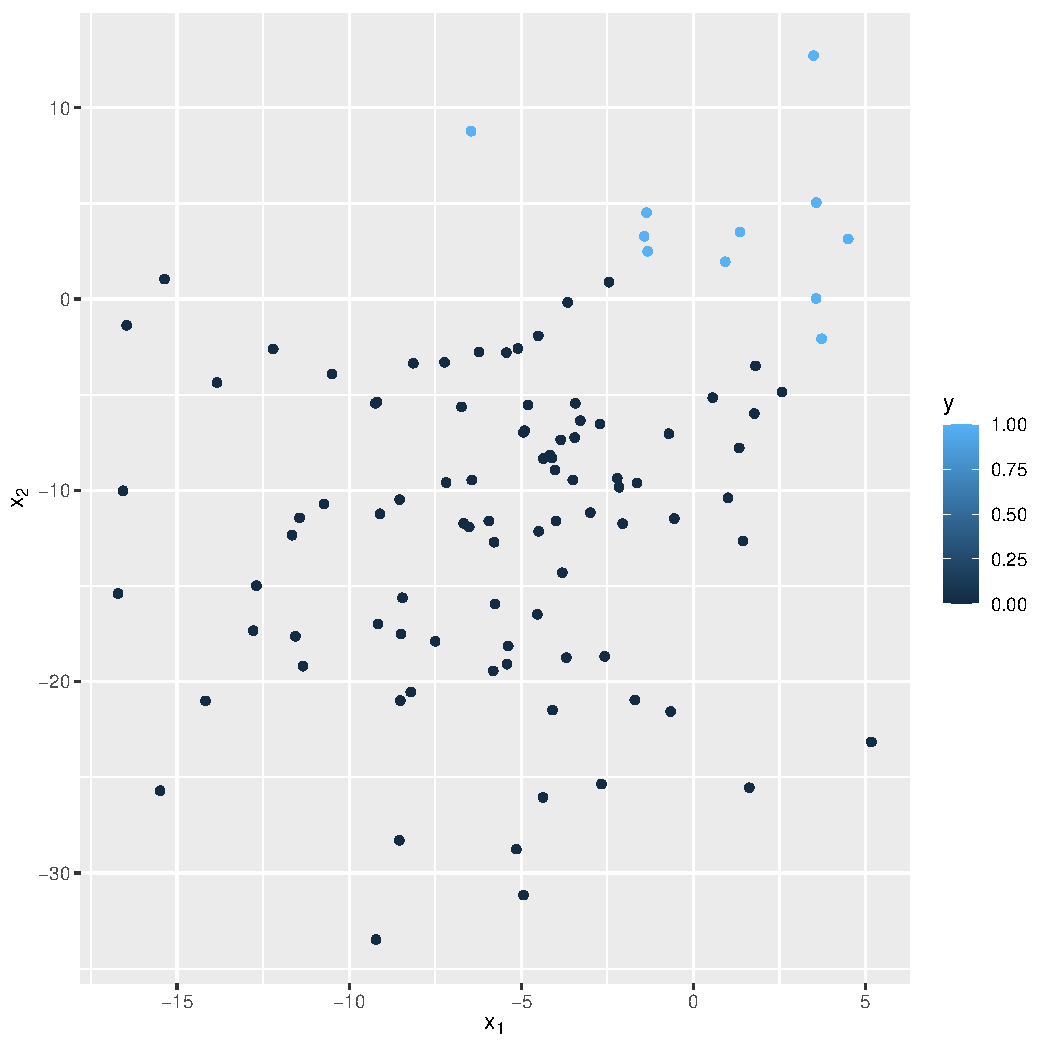
\includegraphics[width=0.5\linewidth]{figure/mv-plot-1} 
\end{knitrout}

\begin{enumerate}
\item
We start with
\begin{align*}
  \mathcal{R}_\text{emp}(\tilde{\bm{\theta}}) &= \sum^n_{i=1} \log(1 + \exp(\tilde{\bm{\theta}}^\top \mathbf{x}^{(i)})) - y^{(i)}\tilde{\bm{\theta}}^\top \mathbf{x}^{(i)} \\
  &= \sum^n_{i=1} \begin{cases}
    \log(1 + \exp(\tilde{\bm{\theta}}^\top \mathbf{x}^{(i)})) & \text{if $y^{(i)} = 0$}, \\
    \log(1 + \exp(\tilde{\bm{\theta}}^\top \mathbf{x}^{(i)})) - \tilde{\bm{\theta}}^\top \mathbf{x}^{(i)} & \text{if $y^{(i)} = 1$}.
  \end{cases}
\end{align*}

Since $\tilde{\bm{\theta}}$ perfectly classifies the data, we know that
\begin{equation*}
  \begin{cases}
    \tilde{\bm{\theta}}^\top \xv^{(i)} < 0 & \text{if $y^{(i)} = 0$}, \\
    \tilde{\bm{\theta}}^\top \xv^{(i)} \geq 0 & \text{if $y^{(i)} = 1$}.
  \end{cases}
\end{equation*}

Hence, we can focus on the functions $g(z) = \log(1 + \exp(-z))$ and $h(z) = \log(1 + \exp(z)) - z$ for $z > 0$ and study their monotonicity.

We compute
\begin{equation*}
  g'(z) = \frac{1}{1 + \exp(-z)} \cdot \exp(-z) \cdot (-1) = - \underbrace{\frac{\exp(-z)}{1 + \exp(-z)}}_{> 0} < 0
\end{equation*}
and
\begin{equation*}
  h'(z) = \underbrace{\frac{\exp(z)}{1 + \exp(z)}}_{< 1} - 1 < 0.
\end{equation*}
Therefore, both $g$ and $h$ are strictly monotonically decreasing.

It follows that $\mathcal{R}_\text{emp}(\tilde{\bm{\theta}}) > \mathcal{R}_\text{emp}(\alpha \tilde{\bm{\theta}})$ for $\alpha > 1$.

\item
\begin{knitrout}
\definecolor{shadecolor}{rgb}{0.969, 0.969, 0.969}\color{fgcolor}\begin{kframe}
\begin{alltt}
\hldef{lambda} \hlkwb{=} \hlnum{0}

\hldef{f} \hlkwb{<-} \hlkwa{function}\hldef{(}\hlkwc{theta}\hldef{,} \hlkwc{lambda}\hldef{) lambda} \hlopt{*} \hldef{theta} \hlopt \hldef{theta} \hlopt{+}
  \hlkwd{sum}\hldef{(}\hlopt{-}\hldef{y} \hlopt{*} \hldef{X} \hlopt \hldef{theta} \hlopt{+} \hlkwd{log}\hldef{(}\hlnum{1} \hlopt{+} \hlkwd{exp}\hldef{(X} \hlopt \hldef{theta)))}

\hldef{x} \hlkwb{=} \hlkwd{seq}\hldef{(}\hlopt{-}\hlnum{1}\hldef{,} \hlnum{5}\hldef{,} \hlkwc{by}\hldef{=}\hlnum{0.1}\hldef{)}
\hldef{xx} \hlkwb{=} \hlkwd{expand.grid}\hldef{(}\hlkwc{X1} \hldef{= x,} \hlkwc{X2} \hldef{= x)}

\hldef{fxx} \hlkwb{=} \hlkwd{log}\hldef{(}\hlkwd{apply}\hldef{(xx,} \hlnum{1}\hldef{,} \hlkwa{function}\hldef{(}\hlkwc{t}\hldef{)} \hlkwd{f}\hldef{(t, lambda)))}
\hldef{df} \hlkwb{=} \hlkwd{data.frame}\hldef{(}\hlkwc{xx} \hldef{= xx,} \hlkwc{fxx} \hldef{= fxx)}

\hlkwd{ggplot}\hldef{()} \hlopt{+}
    \hlkwd{geom_contour_filled}\hldef{(}\hlkwc{data} \hldef{= df,} \hlkwd{aes}\hldef{(}\hlkwc{x} \hldef{= xx.X1,} \hlkwc{y} \hldef{= xx.X2,} \hlkwc{z} \hldef{= fxx))} \hlopt{+}
    \hlkwd{xlab}\hldef{(}\hlkwd{expression}\hldef{(theta[}\hlnum{1}\hldef{]))} \hlopt{+}
    \hlkwd{ylab}\hldef{(}\hlkwd{expression}\hldef{(theta[}\hlnum{2}\hldef{]))}
\end{alltt}
\end{kframe}
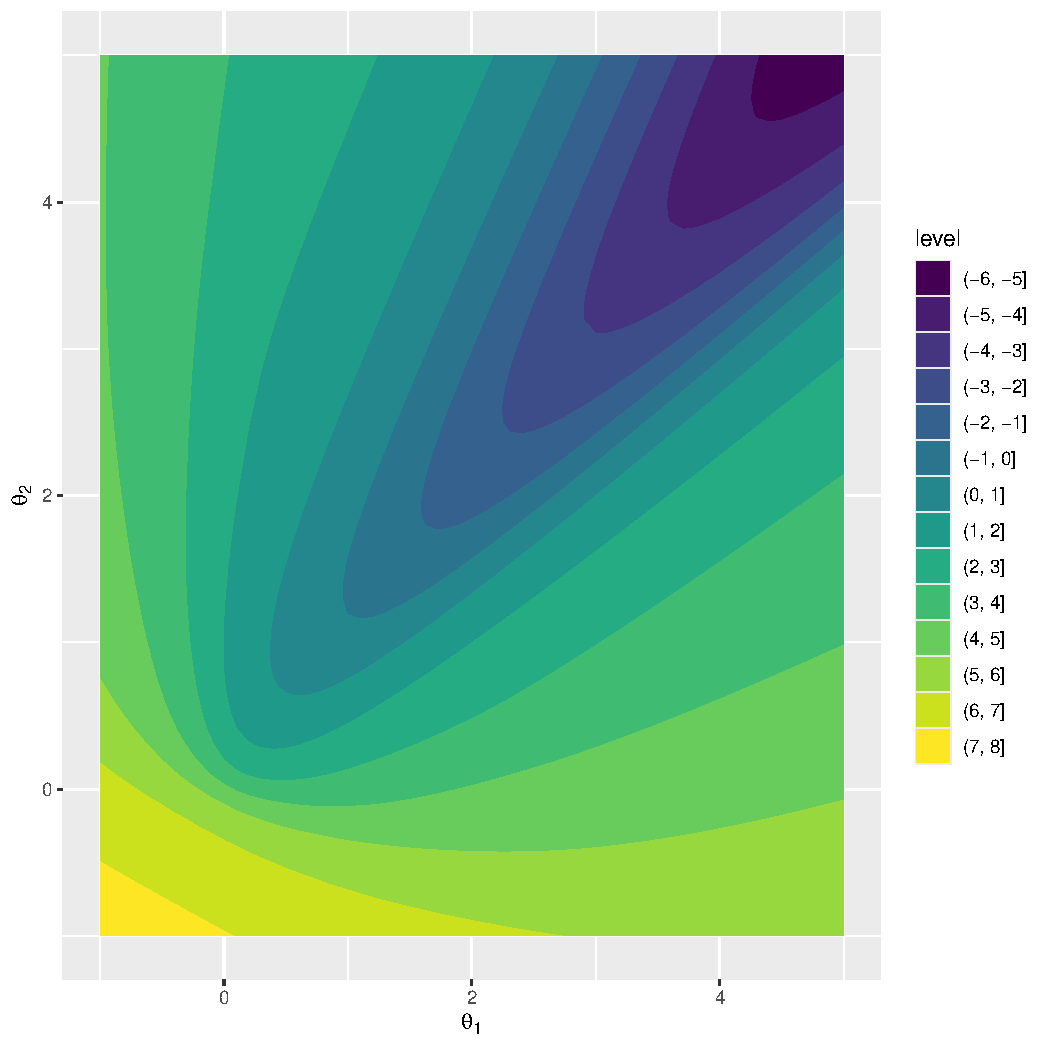
\includegraphics[width=0.5\linewidth]{figure/mv-plot_r_emp-1} 
\end{knitrout}

\item $\frac{\partial}{\partial \bm{\theta}}\mathcal{R}_{\text{emp}} = \sum^n_{i=1} \frac{\exp(\bm{\theta}^\top \mathbf{x}^{(i)})}{1 + \exp(\bm{\theta}^\top \mathbf{x}^{(i)})}{\mathbf{x}^{(i)}}^\top - y^{(i)}{\mathbf{x}^{(i)}}^\top$ 
\item Note that we visualize form the first iteration on ($t = 1$) and not from the initial starting point $\bm{\theta}^{[0]} = (0,0)^\top$ but after having already made one GD step.

\begin{knitrout}
\definecolor{shadecolor}{rgb}{0.969, 0.969, 0.969}\color{fgcolor}\begin{kframe}
\begin{alltt}
\hlkwd{library}\hldef{(gridExtra)}

\hldef{plot_fun} \hlkwb{<-} \hlkwa{function}\hldef{(}\hlkwc{gd_fun}\hldef{,} \hlkwc{lambda}\hldef{)\{}
  \hldef{theta} \hlkwb{=} \hlkwd{c}\hldef{(}\hlnum{0}\hldef{,}\hlnum{0}\hldef{)}
  \hldef{thetas} \hlkwb{=} \hlkwa{NULL}
  \hldef{thetas_norm} \hlkwb{=} \hlkwa{NULL}
  \hldef{fs} \hlkwb{=} \hlkwa{NULL}
  \hlkwa{for}\hldef{(i} \hlkwa{in} \hlnum{1}\hlopt{:}\hlnum{500}\hldef{)\{}
    \hldef{theta} \hlkwb{=} \hlkwd{gd_fun}\hldef{(theta)}
    \hldef{thetas_norm} \hlkwb{=} \hlkwd{rbind}\hldef{(thetas_norm,} \hlkwd{sqrt}\hldef{(theta} \hlopt \hldef{theta))}
    \hldef{thetas} \hlkwb{=} \hlkwd{rbind}\hldef{(thetas,} \hlkwd{t}\hldef{(theta))}
    \hldef{fs} \hlkwb{=} \hlkwd{rbind}\hldef{(fs,} \hlkwd{f}\hldef{(theta, lambda))}
  \hldef{\}}

  \hldef{df_trace} \hlkwb{=} \hlkwd{as.data.frame}\hldef{(thetas)}
  \hldef{df_trace}\hlopt{$}\hldef{t} \hlkwb{=} \hlnum{1}\hlopt{:}\hlkwd{nrow}\hldef{(df_trace)}
  \hldef{trace_plot} \hlkwb{=} \hlkwd{ggplot}\hldef{()} \hlopt{+}
    \hlkwd{geom_point}\hldef{(}\hlkwc{data} \hldef{= df_trace,} \hlkwd{aes}\hldef{(}\hlkwc{x}\hldef{=V1,} \hlkwc{y}\hldef{=V2,} \hlkwc{colour}\hldef{=t))} \hlopt{+}
    \hlkwd{xlab}\hldef{(}\hlkwd{expression}\hldef{(theta[}\hlnum{1}\hldef{]))} \hlopt{+}
    \hlkwd{ylab}\hldef{(}\hlkwd{expression}\hldef{(theta[}\hlnum{2}\hldef{]))}
  \hldef{norm_plot} \hlkwb{=} \hlkwd{ggplot}\hldef{(}\hlkwd{data.frame}\hldef{(}\hlkwc{norms} \hldef{= thetas_norm,} \hlkwc{t} \hldef{=} \hlnum{1}\hlopt{:}\hlkwd{nrow}\hldef{(thetas_norm)))} \hlopt{+}
    \hlkwd{geom_line}\hldef{(}\hlkwd{aes}\hldef{(}\hlkwc{x} \hldef{= t,} \hlkwc{y} \hldef{= norms))} \hlopt{+}
    \hlkwd{scale_x_continuous}\hldef{(}\hlkwc{breaks} \hldef{=} \hlkwd{c}\hldef{(}\hlnum{1}\hldef{,} \hlnum{100}\hldef{,} \hlnum{200}\hldef{,} \hlnum{300}\hldef{,} \hlnum{400}\hldef{,} \hlnum{500}\hldef{),} \hlkwc{limits} \hldef{=} \hlkwd{c}\hldef{(}\hlnum{1}\hldef{,} \hlnum{500}\hldef{))} \hlopt{+}
    \hlkwd{ylab}\hldef{(}\hlkwd{expression}\hldef{(}\hlkwd{paste}\hldef{(}\hlsng{"||"}\hldef{, theta,} \hlsng{"||"}\hldef{[}\hlnum{2}\hldef{])))}
  \hldef{remp_plot} \hlkwb{=} \hlkwd{ggplot}\hldef{(}\hlkwd{data.frame}\hldef{(}\hlkwc{f} \hldef{= fs,} \hlkwc{t} \hldef{=} \hlnum{1}\hlopt{:}\hlkwd{nrow}\hldef{(thetas_norm)))} \hlopt{+}
    \hlkwd{geom_line}\hldef{(}\hlkwd{aes}\hldef{(}\hlkwc{x} \hldef{= t,} \hlkwc{y} \hldef{= f))} \hlopt{+}
    \hlkwd{scale_x_continuous}\hldef{(}\hlkwc{breaks} \hldef{=} \hlkwd{c}\hldef{(}\hlnum{1}\hldef{,} \hlnum{100}\hldef{,} \hlnum{200}\hldef{,} \hlnum{300}\hldef{,} \hlnum{400}\hldef{,} \hlnum{500}\hldef{),} \hlkwc{limits} \hldef{=} \hlkwd{c}\hldef{(}\hlnum{1}\hldef{,} \hlnum{500}\hldef{))} \hlopt{+}
    \hlkwd{ylab}\hldef{(}\hlkwd{expression}\hldef{(R[emp]))}
  \hlkwd{grid.arrange}\hldef{(trace_plot, norm_plot, remp_plot,} \hlkwc{ncol}\hldef{=}\hlnum{3}\hldef{)}
\hldef{\}}

\hldef{df_t} \hlkwb{<-} \hlkwa{function}\hldef{(}\hlkwc{theta}\hldef{,} \hlkwc{lambda}\hldef{) lambda} \hlopt{*} \hlkwd{t}\hldef{(theta)} \hlopt{-}\hldef{(}\hlkwd{t}\hldef{(y)} \hlopt \hldef{X)} \hlopt{+}
  \hlkwd{t}\hldef{(}\hlnum{1}\hlopt{/}\hldef{(}\hlnum{1} \hlopt{+} \hlkwd{exp}\hldef{(}\hlopt{-}\hldef{X} \hlopt \hldef{theta)))} \hlopt \hldef{X}

\hldef{gd_step} \hlkwb{<-} \hlkwa{function}\hldef{(}\hlkwc{theta}\hldef{,} \hlkwc{alpha}\hldef{,} \hlkwc{lambda}\hldef{)} \hlkwd{return}\hldef{(theta} \hlopt{-} \hldef{alpha} \hlopt{*} \hlkwd{df_t}\hldef{(theta, lambda)[}\hlnum{1}\hldef{,])}

\hlcom{## Alpha = 0.01}
\hldef{gd_fun} \hlkwb{<-} \hlkwa{function}\hldef{(}\hlkwc{theta}\hldef{)} \hlkwd{return}\hldef{(}\hlkwd{gd_step}\hldef{(theta,} \hlnum{0.01}\hldef{, lambda))}
\hlkwd{plot_fun}\hldef{(gd_fun,} \hlnum{0}\hldef{)}
\end{alltt}
\end{kframe}
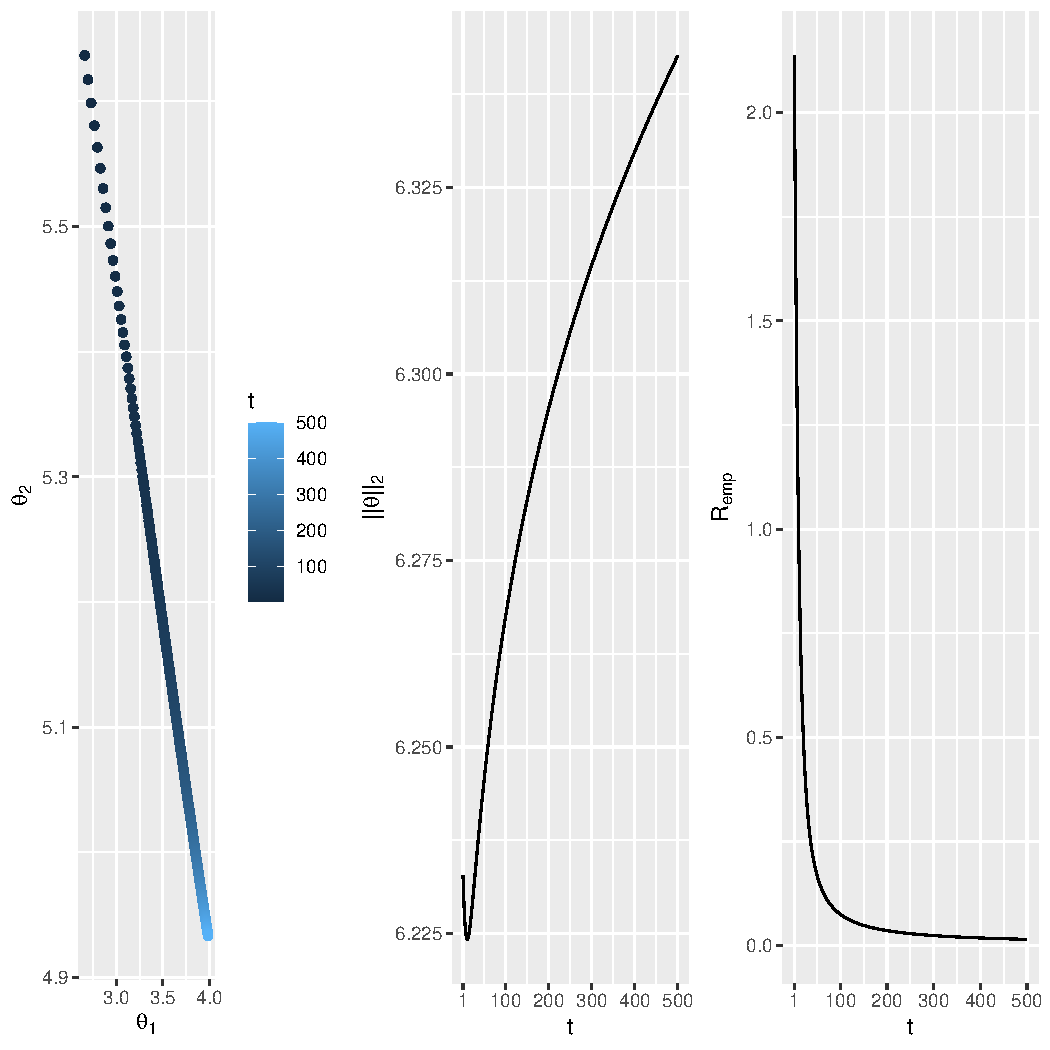
\includegraphics[width=0.5\linewidth]{figure/mv-plot_gd_step-1} 
\begin{kframe}\begin{alltt}
\hlcom{## Alpha = 0.02}
\hldef{gd_fun} \hlkwb{<-} \hlkwa{function}\hldef{(}\hlkwc{theta}\hldef{)} \hlkwd{return}\hldef{(}\hlkwd{gd_step}\hldef{(theta,} \hlnum{0.02}\hldef{, lambda))}
\hlkwd{plot_fun}\hldef{(gd_fun,} \hlnum{0}\hldef{)}
\end{alltt}
\end{kframe}
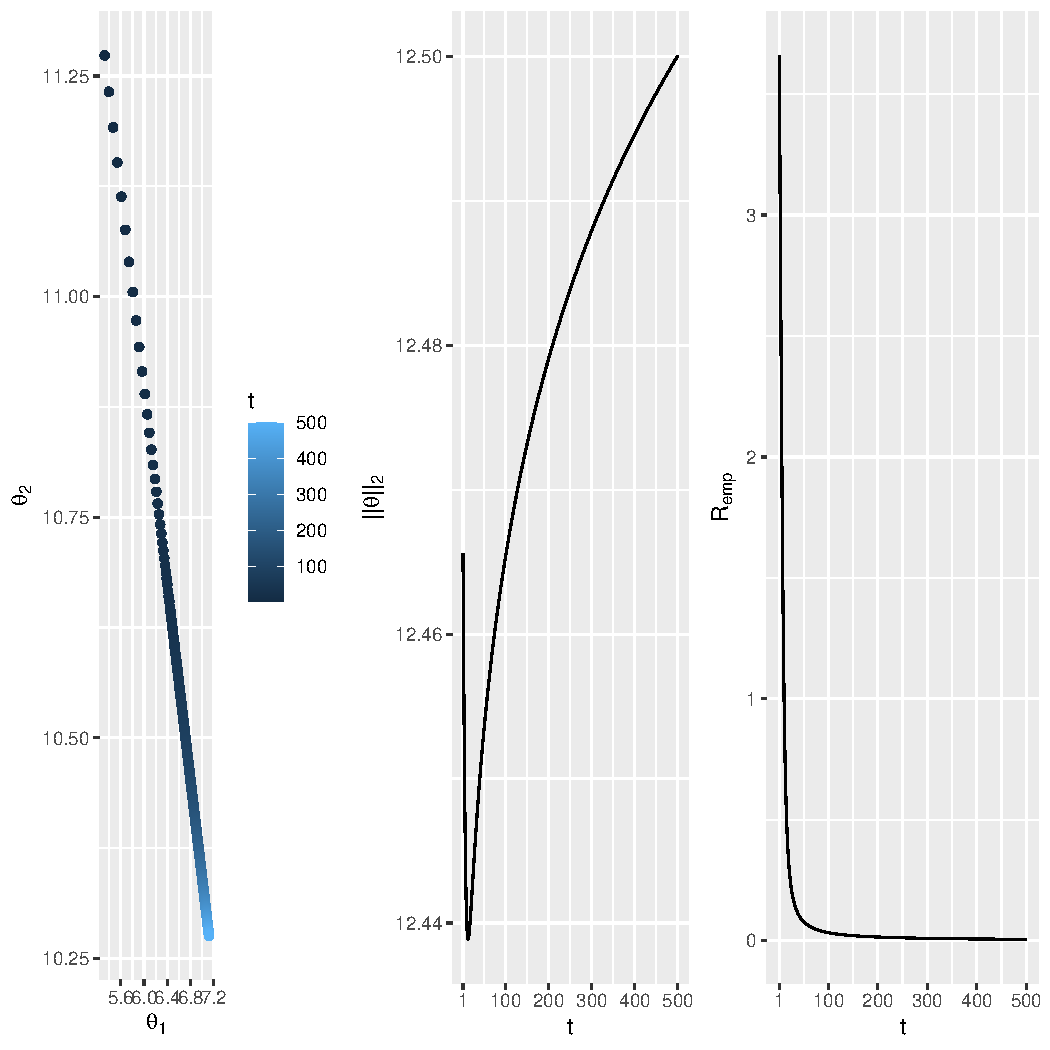
\includegraphics[width=0.5\linewidth]{figure/mv-plot_gd_step-2} 
\end{knitrout}

Gradient descent will in theory not converge since $\mathcal{R}_\text{emp}$ has no minimum (a)
\item

\begin{knitrout}
\definecolor{shadecolor}{rgb}{0.969, 0.969, 0.969}\color{fgcolor}\begin{kframe}
\begin{alltt}
\hlcom{## Lambda = 1, alpha = 0.01}
\hldef{gd_fun} \hlkwb{<-} \hlkwa{function}\hldef{(}\hlkwc{theta}\hldef{)} \hlkwd{return}\hldef{(}\hlkwd{gd_step}\hldef{(theta,} \hlnum{0.01}\hldef{,} \hlnum{1}\hldef{))}
\hlkwd{plot_fun}\hldef{(gd_fun,} \hlnum{1}\hldef{)}
\end{alltt}
\end{kframe}
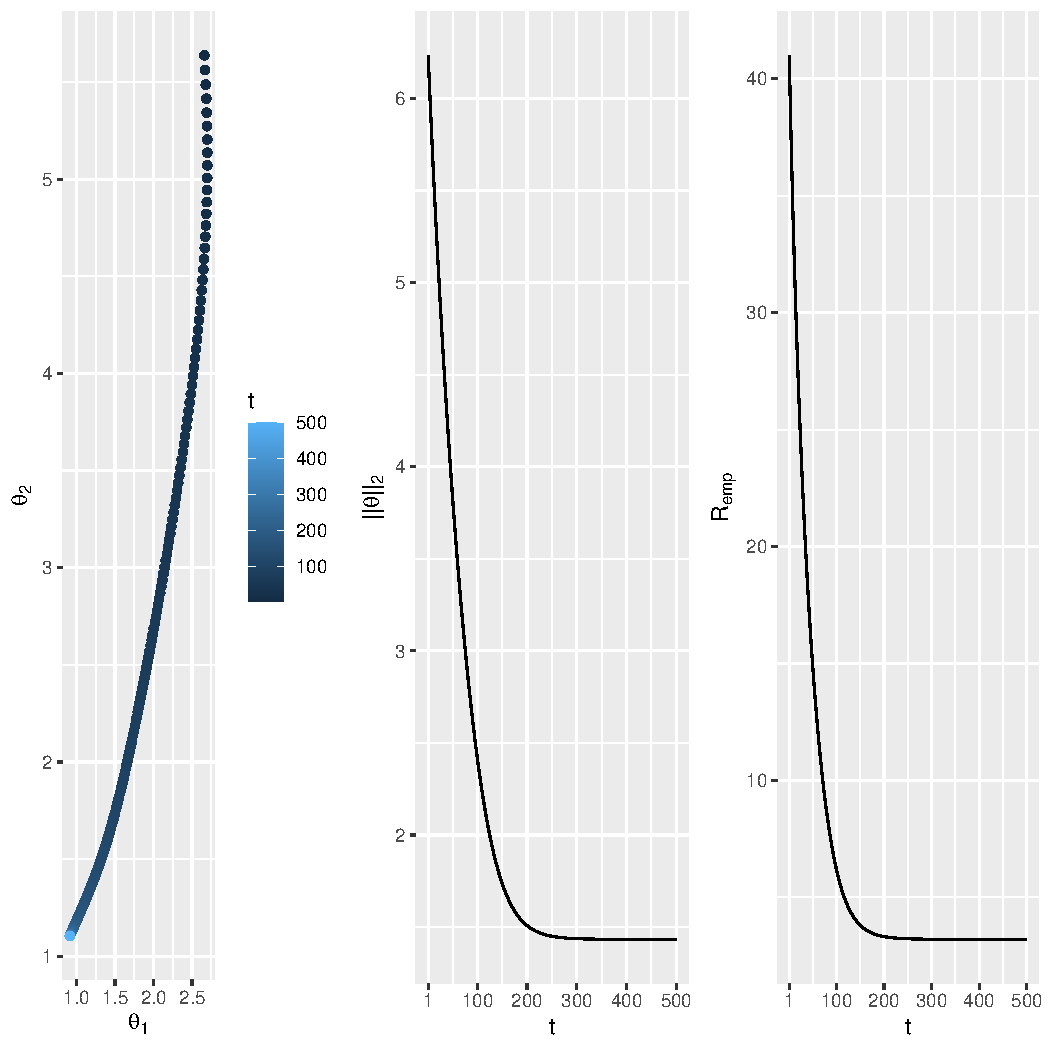
\includegraphics[width=0.5\linewidth]{figure/mv-plot_gd_step_reg-1} 
\begin{kframe}\begin{alltt}
\hlcom{## Lambda = 1, alpha = 0.02}
\hldef{gd_fun} \hlkwb{<-} \hlkwa{function}\hldef{(}\hlkwc{theta}\hldef{)} \hlkwd{return}\hldef{(}\hlkwd{gd_step}\hldef{(theta,} \hlnum{0.02}\hldef{,} \hlnum{1}\hldef{))}
\hlkwd{plot_fun}\hldef{(gd_fun,} \hlnum{1}\hldef{)}
\end{alltt}
\end{kframe}
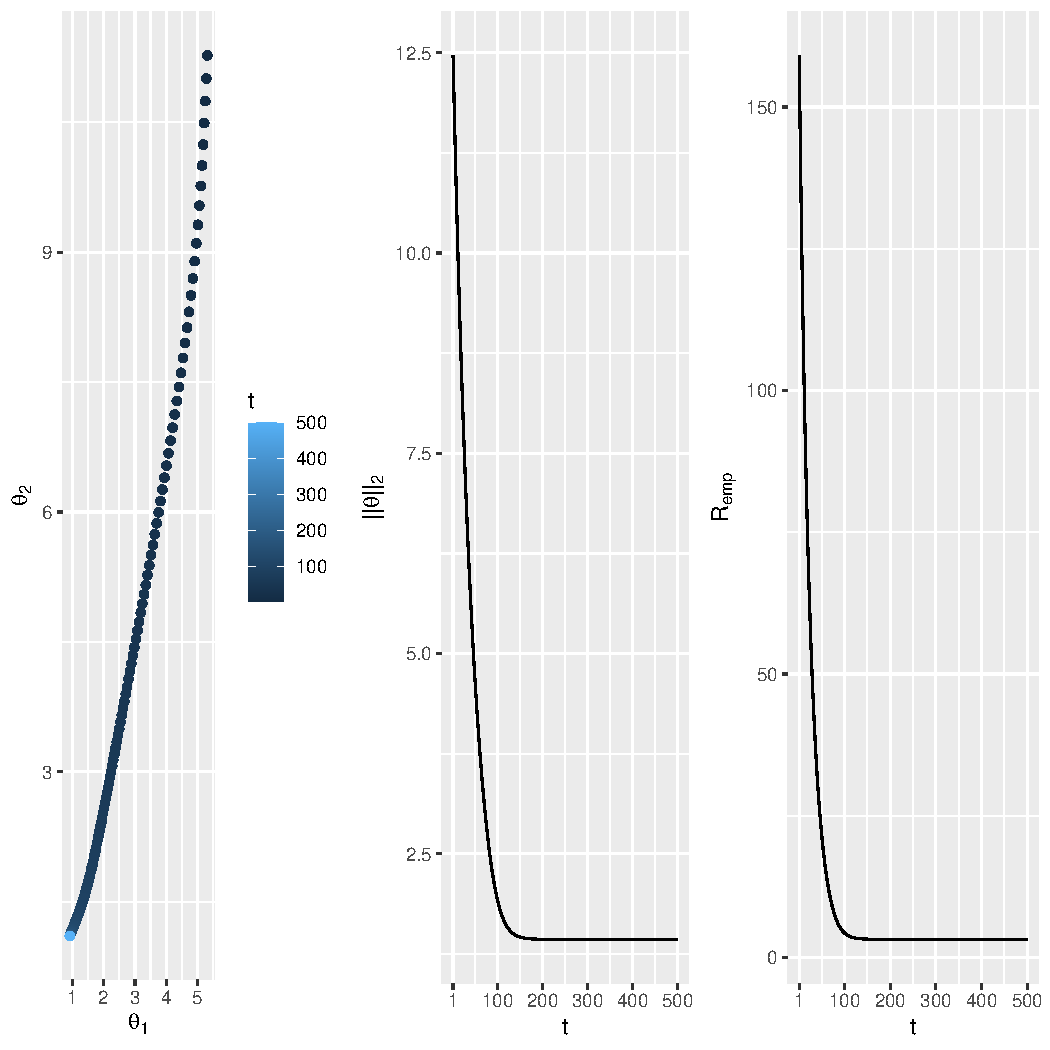
\includegraphics[width=0.5\linewidth]{figure/mv-plot_gd_step_reg-2} 
\end{knitrout}

\item 
\begin{knitrout}
\definecolor{shadecolor}{rgb}{0.969, 0.969, 0.969}\color{fgcolor}\begin{kframe}
\begin{alltt}
\hldef{lambda} \hlkwb{=} \hlnum{1}

\hldef{fxx_reg} \hlkwb{=} \hlkwd{log}\hldef{(}\hlkwd{apply}\hldef{(xx,} \hlnum{1}\hldef{,} \hlkwa{function}\hldef{(}\hlkwc{t}\hldef{)} \hlkwd{f}\hldef{(t, lambda)))}
\hldef{df_reg} \hlkwb{=} \hlkwd{data.frame}\hldef{(}\hlkwc{xx} \hldef{= xx,} \hlkwc{fxx} \hldef{= fxx_reg)}

\hlkwd{ggplot}\hldef{()} \hlopt{+}
    \hlkwd{geom_contour_filled}\hldef{(}\hlkwc{data} \hldef{= df_reg,} \hlkwd{aes}\hldef{(}\hlkwc{x} \hldef{= xx.X1,} \hlkwc{y} \hldef{= xx.X2,} \hlkwc{z} \hldef{= fxx))} \hlopt{+}
    \hlkwd{xlab}\hldef{(}\hlkwd{expression}\hldef{(theta[}\hlnum{1}\hldef{]))} \hlopt{+}
    \hlkwd{ylab}\hldef{(}\hlkwd{expression}\hldef{(theta[}\hlnum{2}\hldef{]))}
\end{alltt}
\end{kframe}
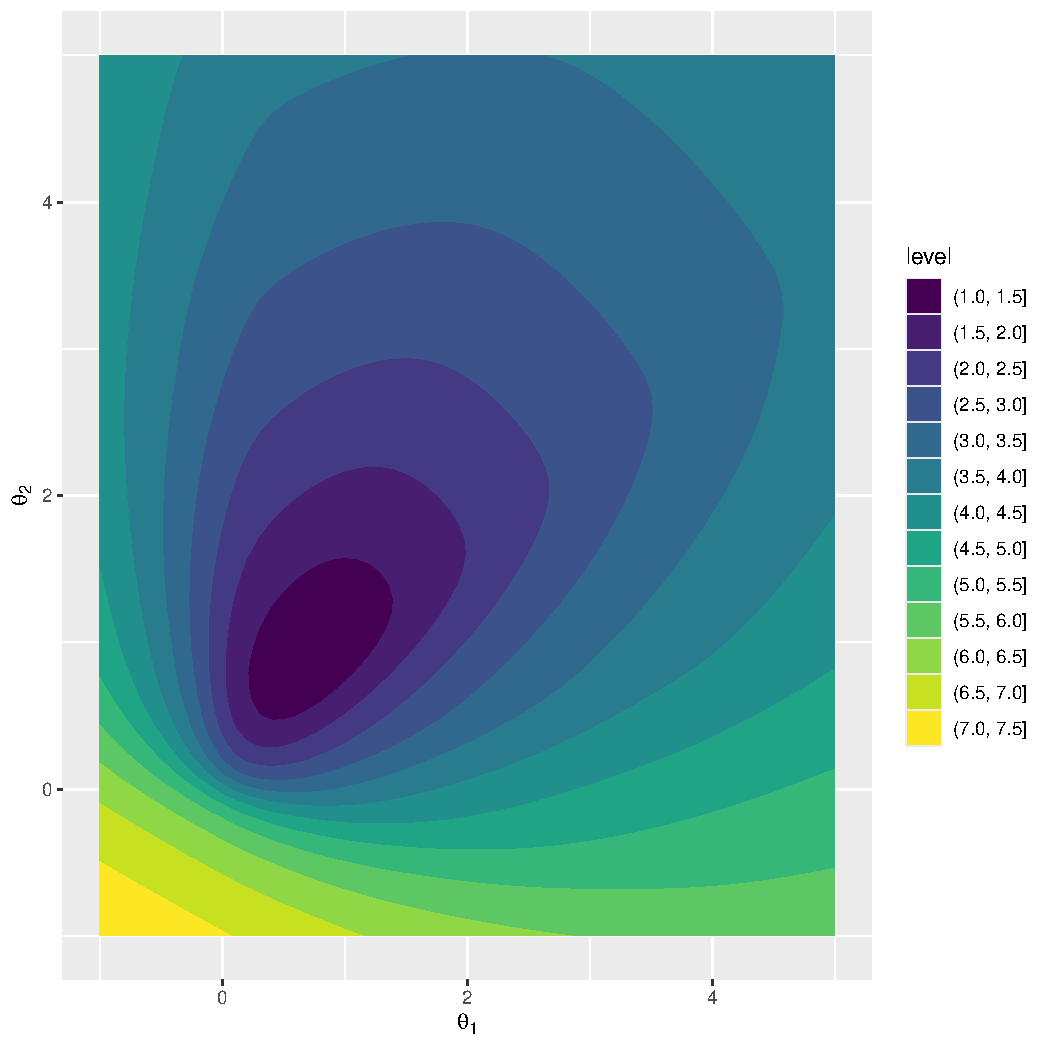
\includegraphics[width=0.5\linewidth]{figure/mv-plot_r_emp_reg-1} 
\end{knitrout}
\item
\begin{knitrout}
\definecolor{shadecolor}{rgb}{0.969, 0.969, 0.969}\color{fgcolor}\begin{kframe}
\begin{alltt}
\hldef{gd_backtracking_step} \hlkwb{<-} \hlkwa{function}\hldef{(}\hlkwc{theta}\hldef{,} \hlkwc{alpha}\hldef{,} \hlkwc{gamma}\hldef{,} \hlkwc{tau}\hldef{,} \hlkwc{lambda}\hldef{)\{}
    \hldef{ftheta} \hlkwb{=} \hlkwd{f}\hldef{(theta, lambda)}
    \hldef{dftheta} \hlkwb{=} \hlkwd{df_t}\hldef{(theta, lambda)[}\hlnum{1}\hldef{,]}
    \hlkwa{for}\hldef{(i} \hlkwa{in} \hlnum{1}\hlopt{:}\hlnum{1000}\hldef{) \{}
      \hldef{theta_prop} \hlkwb{=} \hldef{theta} \hlopt{-} \hldef{alpha} \hlopt{*} \hldef{dftheta}
      \hlkwa{if}\hldef{(}\hlkwd{f}\hldef{(theta_prop, lambda)} \hlopt{<=} \hldef{ftheta} \hlopt{-} \hldef{gamma} \hlopt{*} \hldef{alpha} \hlopt{*} \hlkwd{t}\hldef{(dftheta)} \hlopt \hldef{dftheta)\{}
        \hlkwd{return}\hldef{(theta_prop)}
      \hldef{\}}\hlkwa{else}\hldef{\{}
        \hldef{alpha} \hlkwb{=} \hldef{tau} \hlopt{*} \hldef{alpha}
      \hldef{\}}
    \hldef{\}}
    \hlkwd{return}\hldef{(theta)}
\hldef{\}}

\hlcom{## Lambda = 1, alpha = 0.01}
\hldef{gd_fun} \hlkwb{<-} \hlkwa{function}\hldef{(}\hlkwc{theta}\hldef{)} \hlkwd{return}\hldef{(}\hlkwd{gd_backtracking_step}\hldef{(theta,} \hlnum{0.01}\hldef{,} \hlnum{0.9}\hldef{,} \hlnum{0.5}\hldef{,} \hlnum{1}\hldef{))}
\hlkwd{plot_fun}\hldef{(gd_fun,} \hlnum{1}\hldef{)}
\end{alltt}
\end{kframe}
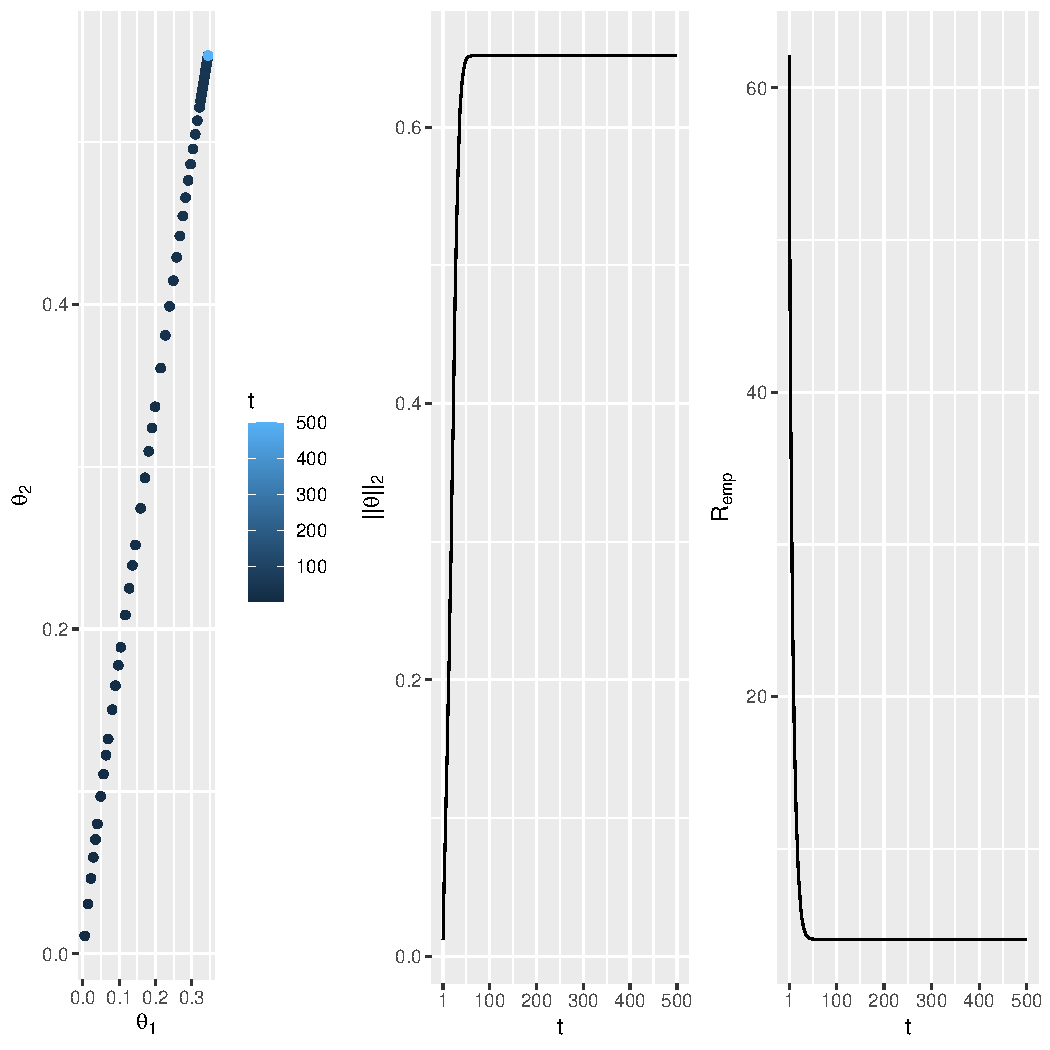
\includegraphics[width=0.5\linewidth]{figure/mv-plot_gd_backtrack-1} 
\begin{kframe}\begin{alltt}
\hlcom{## Lambda = 1, alpha = 0.02}
\hldef{gd_fun} \hlkwb{<-} \hlkwa{function}\hldef{(}\hlkwc{theta}\hldef{)} \hlkwd{return}\hldef{(}\hlkwd{gd_backtracking_step}\hldef{(theta,} \hlnum{0.02}\hldef{,} \hlnum{0.9}\hldef{,} \hlnum{0.5}\hldef{,} \hlnum{1}\hldef{))}
\hlkwd{plot_fun}\hldef{(gd_fun,} \hlnum{1}\hldef{)}
\end{alltt}
\end{kframe}
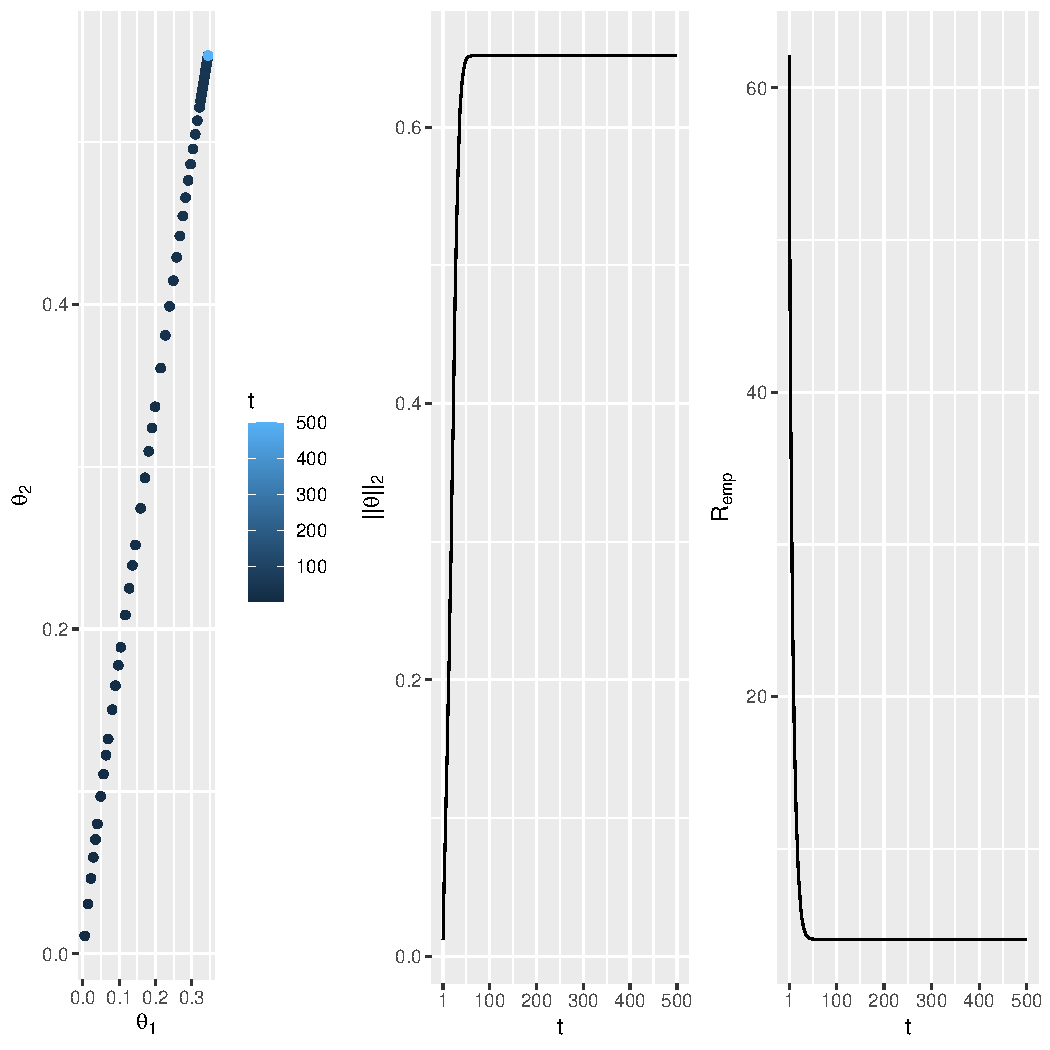
\includegraphics[width=0.5\linewidth]{figure/mv-plot_gd_backtrack-2} 
\end{knitrout}
\end{enumerate}
}
\end{document}
